\section{Аналитическая часть}

В данной части будет рассмотрена предметная область параллельных корпусов текстов, будут описаны виды текстовых разметок, структура научно-технических текстов и проблемы, возникающие при попытке автоматизации выравнивания текстов на уровне терминов.

\subsection{Корпуса текстов}

Одним из направлений корпусной лингвистики является создание и использование параллельных корпусов, которые используются для решения различных задач, таких как создание и настройка систем машинного перевода, сравнительное изучение языков, разработка теории переводческих исследований, преподавания языка~\cite{butenko2020-9}.
Корпусы и конкордансы предоставляют лингвистам, переводчикам и студентам бесценный и ранее недоступный языковой материал, который характеризуется большим объемом, разнообразием стилей и жанров и возможностью быстрого поиска примеров проанализированных слов и конструкций.~\cite{butenko2020-1}

Следует отметить, что под корпусом параллельных текстов понимается тип лингвистического корпуса, состоящий из исходного текста на одном языке и его перевода на другой или другие языки, а конкорданс --- одна из программ, которая позволяет обрабатывать и анализировать большие массивы текста, а также выявлять языковые шаблоны, которые в них содержатся.
Конкорданс ищет конкретное слово или выражение в корпусе.
После соответствующей команды программа выдает указанное количество текстовых фрагментов, содержащих нужные единицы измерения.
На основании полученной информации возможно определить, какие функции, применение и использование устройства были определены в конкретном языковом пространстве.~\cite{butenko2020-1}

\subsubsection{Виды}

В отличие от других типов корпусов, отличительным дидактическим свойством корпусов параллельных текстов является многоязычие.

Корпусы параллельных текстов могут быть двуязычные и многоязычные.
Двуязычные корпусы включают исходные тексты на одном языке и их переводы на другом.
Многоязычные корпусы включают исходные текста на одном языке и их соответствующие переводы на другие языки.

Корпусы могут быть однонаправленные, двунаправленные и многонаправленные.
Однонаправленные корпусы позволяют осуществлять перевод с одного языка на другой (например, с английского на русский) без возможности обратного перевода (с русского на английский).
Двунаправленные корпусы включают параллельные тексты на двух языках (английском и русском) и позволяют осуществлять перевод как с английского на русский, так и наоборот).
Многонаправленные корпусы, включающие тексты на более чем двух языках, позволяют осуществлять перевод с любого языка на любой (в рамках существующих языков корпуса).

Параллельный корпус имеет много общего с памятью переводов, но разница в том, что память переводов не сохраняет оригинальную последовательность текста, тогда как параллельные тексты — сохраняют.~\cite{butenko2020-1}

\subsubsection{Применение}

Параллельные корпусы используются: 
\begin{enumerate}
    \item в сравнительной лингвистике: для сравнительного анализа структур двух языков; 
    \item в области переводов; для поиска эквивалентов оригинального текста в других языках; 
    \item при обучении движков машинного перевода; 
    \item при изучении языка; 
    \item при составлении словарей. 
\end{enumerate}

Практика разработки и использования электронных текстовых корпусов показала, что создать универсальный корпус невозможно.
Цели и задачи любого исследования, которое предполагается выполнить с помощью корпусов, определяют тип корпуса, правила отбора текстов, метод и степень обработки.
В области корпусной лингвистики уже создано большое количество корпусов, предназначенных для различных видов исследований, и задача их классификации требует определения различных характеристик --- основы классификации.

Параллельные корпусы, представляющие множество текстов-оригиналов, написанных на каком-либо исходном языке, и переводов этих исходных текстов на один или несколько других языков; правда, существуют корпусы, в которых все языки признаются равнозначными, например, корпусы, созданные на основе официальных документов ООН или Европейского Сообщества.

Параллельные корпусы используются для разработки эффективных  методов перевода, а также для сравнительных исследований языков.
Он позволяет идентифицировать те или иные приемы перевода, оценить их эффективность, проанализировать лексику и грамматику текста перевода в сопоставлении с оригинальным текстом, сравнить и оценить различные стратегии перевода, найти на основе списков контекстов соответствия тем или иным стилистическим явлениям и выделить способы их передачи при переводе.~\cite{butenko2020-1}

\subsection{Тексты}

Тексты корпусов обычно размечаются для удобства пользования, т. е. текстам и содержащимся в них языковым единицам приписываются специальные метки.
Размеченные корпуса обеспечивают специализированными поисковыми системами, реализующими грамматические и лексические виды поиска.
В зависимости о целей создания корпуса в него включают дополнительные виды разметки.~\cite{butenko2020-2}

\subsubsection{Виды разметок}

Разметка (tagging, annotation) корпуса лексикографических материалов заключается в приписывании источникам и их компонентам специальных лингвистических и экстралингвистических тэгов (токенов).
Именно разметка позволяет идентифицировать первоисточники и обеспечивает семантический, осмысленный, расширенный поиск по различным тегам, параметрам и критериям.~\cite{lesnikov2019}

Различают следующие виды разметок:
\begin{itemize}
    \item морфологическая (part-of-speech tagging; грамматическая, частеречная; парсер) --- включает не только признак части речи, но и признаки грамматических категорий, свойственных данной части речи, т. е. в том или ином структурированном виде включаются лемма, признак части речи и признаки грамматических категорий (граммемы --- падеж, переходность, род, одушевленность, число). Морфологический анализ корпуса текстов может заключаться: в токенизации (разбиении на орфографические слова, элементарные знаки --- токены); в сегментации (на предложения, клаузулы и др. виды сегментов); в лемматизации (нормализация словоформ, т. е. сведение различных словоформ к некоторому единому представлению --- к исходной форме, или лемме); в стемминге (нормализация словоформ, когда разные словоформы приводятся к <<псевдооснове>> или усекаются до их корневой части, для отражения инвариантного значения слова); в частеречном тэгинге (pos-tagging, т. е. указание части речи для каждой словоформы в тексте) или в полном морфологическом анализе --- приписывании грамматических характеристик всем словоформам; в построении гипотез для нераспознанных слов; 
    % \item синтаксическая --- является результатом парсинга, выполняемого программно в автоматизированном режиме на основе данных морфологического анализа, описывает синтаксические связи между лексическими единицами и различные синтаксические конструкции;
    \item семантическая --- приписывает единицам текста один или несколько семантических и словообразовательных признаков; предусматривает спецификацию значения слов, разрешение омонимии и синонимии, категоризацию слов (разряды, родовые и видовые дескрипторы), выделение тематических классов, признаков каузативности, оценочных и деривационных характеристик, семантических ролей (например, агенс, инструмент, пациенс, результат);
    \item структурная --- эксплицирует логическую структуру источника и предназначена для выделения структурных элементов (том, книга, часть, глава, действие, явление, реплика, сноска, ремарка, строфа, стих, а также: абзац, предложение, словоформа и текстоформа; таблица, формула и др.);
    \item терминологическая --- предназначена для фиксации терминов и особенности использования общеупотребительной лексики;
    \item экстралингвистическая (метаразметка метаданных) --- включает внешнюю разметку, формальную структурную разметку, а также технико-технологическую разметку (кодировку, даты обработки, исполнителей, источник электронной версии);
    \item и др.~\cite{lesnikov2019}
\end{itemize}

% \subsubsection*{Морфологическая}

% \subsubsection*{Синтаксическая}

% \subsubsection*{Семантическая}

% \subsubsection*{Метаразметка}

\subsubsection{Структура научно-технических текстов}

Композиционная структура учебно-научного текста в первом приближении состоит из реферативного раздела, корпуса научно-технической статьи и информативного раздела.
При этом структурные элементы научно-учебных текстов можно разделить на обязательные и факультативные, то есть те, которые приводятся в зависимости от необходимости.~\cite{butenko2021}

В нотациях Бекуса-Наура композиционную структуру учебно-научных текстов можно задать следующим образом:

$$
St_{i} ::= \langle X^{1}, X^{2}, X^{3}\rangle ,
$$
где $ X^{1} $ — реферативный раздел учебно-научного текста, $ X^{2} $ — корпус учебно-научного текста, $ X^{3} $ — информативный раздел научно-учебного текста.

$ X^{1} $ — реферативный раздел учебно-научного текста, состоящий из следующих элементов:

$$
X^{1} ::= \langle x_{11}, x_{12}, x_{13}, x_{14}, x_{15}\rangle |\langle x_{11}, x_{12}, x_{13}, x_{14}\rangle ,
$$
где $ x_{11} $ — название, $ x_{12} $ — автор(ы), $ x_{13} $ — оглавление, $ x_{14} $ — введение, $ x_{15} $ — предисловие.

$ X^{2} $ — корпус учебно-научного текста, который можно представить в виде набора из следующих элементов:

$$
X^{2} ::= \langle x_{21}, x_{22}, x_{23}\rangle |\langle x_{21}, x_{22}\rangle |\langle x_{21}, x_{23}\rangle |\langle x_{21}\rangle ,
$$
где $ x_{21} $ — основной текст, $ x_{22} $ — вопросы, $ x_{23} $ — задания и упражнения.

$ X^{3} $ — информативный раздел учебно-научного текста, для которого справедливо

$$
X^{3} ::= \langle x_{31}, x_{32}, x_{33}\rangle |\langle x_{31}, x_{33}\rangle |\langle x_{32}, x_{33}\rangle |\langle x_{33}\rangle ,
$$
где $ x_{31} $ — приложения, $ x_{32} $ — приложения, $ x_{33} $ — ссылки на источник.

На рисунке \ref{fig:ts} представлена структурная схема элементов учебно-научного текста. 

\begin{figure}[H]
	\centering
	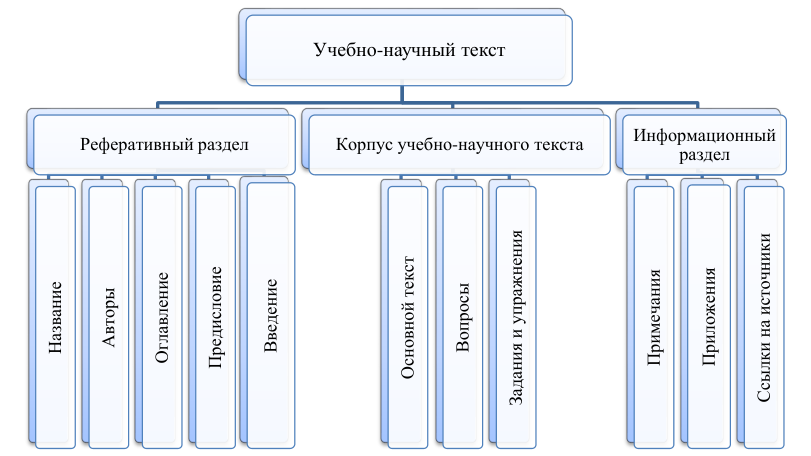
\includegraphics[width=0.9\textwidth]{img/tagging-struct.png}
	\caption{Структурные элементы учебно-научных текстов}
	\label{fig:ts}
\end{figure}

На основе проведенного анализа композиционной структуры учебно-научных текстов модель учебно-научного текста $St$ целесообразно представить в виде: 
$$
St = \langle E^L, R \rangle,
$$
где $E$~---~структурный элемент, $R$~---~отношения между структурными элементами, $L$~---~уровень структурного элемента.
При этом $L = \{l1, \dots l5\}$, где l1~---~раздел, l2~---~ пункт,  l3~---~подпункт, l4 ~---~абзац, l5~---~ предложение.~\cite{butenko2021}

Представление текста в виде упорядоченного набора структурных элементов дает возможность анализировать с помощью математических методов как вероятностную, так и логическую структуру всего учебно-научного текста.

Таким образом, модель композиционной структуры учебно-научного текста --- это граф, вершинами и ребрами которого являются только полноценные единицы --- разделы, пункты, подпункты, то есть наиболее значимые структурные элементы.~\cite{butenko2021}

\newpage

\subsubsection{Проблема терминов}

В ходе исследования \cite{butenko2022} были выделены основные проблемы при автоматическом извлечении терминов:
\begin{itemize}
    \item неправильное определение границ терминов-словосочетаний, состоящих из двух и более слов и составных терминов; 
    \item  распознавание составных терминов и терминов-словосочетаний, состоящих из двух и более слов; в частности, распознавание лексической единицы как части составного термина или как свободной лексической единицы; 
    \item определение лексической единицы как термина в зависимости от контекста и тематики текста, в котором данная лексическая единица употребляется; 
    \item объемные списки терминов-кандидатов, которые необходимо проверять вручную, поскольку частота не является достаточным критерием для оценки того, является ли выделенное слово термином или нет. 
\end{itemize}

Точность определения границ термина при автоматической разметки является одной из основных лингвистических задач. Более того, на сегодняшний день существует малое количество бесплатных ресурсов, а также отсутствуют веб-платформ для автоматической разметки русскоязычных текстов.~\cite{butenko2022}

\subsection{Вывод}

В данной части была рассмотрена предметная область параллельных корпусов текстов, были описаны виды текстовых разметок, структура научно-технических текстов и проблемы, возникающие при попытке автоматизации выравнивания текстов на уровне терминов.
